\documentclass{include/protokollclass}
% Main File - Based on protokollclass.cls
% Comments are mostly in English (and some in German, concerning the Praktikum)
% ------------------------------------------------------------------------------
% Further files in folder:
%  - include/cmds.tex (for macros and additional commands)
%  - include/kitlogo.pdf (for titlepage)
%  - lit.bib (bibtex bibliography database)
%  - include/titlepage.tex (for layout of titelpage)
% ------------------------------------------------------------------------------
% Useful Supplied Packages:
% amsmath, amssymb, mathtools, bbm, upgreek, nicefrac,
% siunitx, varioref, booktabs, graphicx, tikz, multicol


\usepackage{pdfpages}
\usepackage{siunitx}
\usepackage{pgfplots}
\usepackage{pgfplotstable}


%% ---------------------------------------------
%% |    Informationen über dieses Protokoll    |
%% ---------------------------------------------
\newcommand{\praktikum}{P1}                % P1 oder P2
\newcommand{\semester}{WS15/16}            % z.B. "WS14/15" oder "SS15"

\newcommand{\wochentag}{Mo}                % Mo, Di, Mi oder Do
\newcommand{\gruppennr}{25}                % Zweistellige Gruppennummer

\newcommand{\nachnamea}{Kosinksi}             % Nachname des ersten Praktikanten
\newcommand{\vornamea}{Daniel}               % Vorname des ersten Praktikanten
\newcommand{\nachnameb}{Petersen}              % Nachname des zweiten Praktikanten
\newcommand{\vornameb}{Patrick}              % Vorname des zweiten Praktikanten

\newcommand{\emailadressen}{patrick.petersen91@gmail.com, daniel.kosinksi1991@gmail.com}
% optionale Angabe von Emailadresse(n) für den Kontakt mit dem Betreuer

\newcommand{\versuch}{Bestimmung von e/m des Elektrons} % Name des Versuchs
\newcommand{\versuchsnr}{75}               % bitte die korrekte Nummer dem 
                                           % Arbeitsplatz am Versuchstag 
                                           % entnehmen
\newcommand{\fehlerrechnung}{Nein}         % Ob Fehlerrechnung im Versuch 
                                           % durchgeführt wurde oder nicht

\newcommand{\betreuer}{Denise Müller}      % Name des zuständigen Betreuers
\newcommand{\durchgefuehrt}{26.10.15}      % Datum, an dem der Versuch 
                                           % durchgeführt wurde





%% --------------------------------------
%% |    Settings for Word Separation    |
%% --------------------------------------
% Help for separation:
% In German package the following hints are additionally available:
% "- = Additional separation
% "| = Suppress ligation and possible separation (e.g. Schaf"|fell)
% "~ = Hyphenation without separation (e.g. bergauf und "~ab)
% "= = Hyphenation with separation before and after
% "" = Separation without a hyphenation (e.g. und/""oder)

% Describe separation hints here:
\hyphenation
{
    über-nom-me-nen an-ge-ge-be-nen
    %Pro-to-koll-in-stan-zen
    %Ma-na-ge-ment  Netz-werk-ele-men-ten
    %Netz-werk Netz-werk-re-ser-vie-rung
    %Netz-werk-adap-ter Fein-ju-stier-ung
    %Da-ten-strom-spe-zi-fi-ka-tion Pa-ket-rumpf
    %Kon-troll-in-stanz
}





% um die Titelseite per PDF-reader auszufüllen. Vorgefertigte Daten
% können in Datei 'data.tex' modifiziert werden.
%\setboolean{forminput}{true}
% um die Anmerkungen zu den Textfeldern anzeigen zu lassen
%\setboolean{showannotations}{true}
% Erneuern der Seitenzahl in jedem Kapitel
%\setboolean{chapResetPageNumb}{true}
% Einbinden der Kapitelnummer in der Seitenzahl
%\setboolean{chapWiseNumb}{true}
% english or ngerman (new german für neue deutsche Rechtschreibung statt german)
\SelectLanguage{ngerman}





%% -----------------------
%% |    Main Document    |
%% -----------------------
\begin{document}
    % Titlepage und ToC
    \FrontMatter

    % coordinates for background border
\newcommand{\diameter}{20}
\newcommand{\xone}{-15}
\newcommand{\xtwo}{160}
\newcommand{\yone}{15}
\newcommand{\ytwo}{-253}

\newcommand{\hoehea}{60}
\newcommand{\hoeheb}{60}




\begin{titlepage}
    % background border
    \begin{tikzpicture}[overlay]
    \draw[color=gray]  
            (\xone mm, \yone mm)
      -- (\xtwo mm, \yone mm)
    arc (90:0:\diameter pt) 
      -- (\xtwo mm + \diameter pt , \ytwo mm) 
        -- (\xone mm + \diameter pt , \ytwo mm)
    arc (270:180:\diameter pt)
        -- (\xone mm, \yone mm);
    \end{tikzpicture}
    
    % KIT logo
    \begin{textblock}{10}[0,0](4.5,2.5)
        
\includegraphics[width=.25\textwidth]{include/kitlogo.pdf}
    \end{textblock}
    \changefont{phv}{m}{n}    % helvetica
    \begin{textblock}{10}[0,0](5.5,2.2)
        \begin{flushright}
            \Large FAKULTÄT FÜR PHYSIK\\Praktikum Klassische Physik
        \end{flushright}
    \end{textblock}
    
    \begin{textblock}{10}[0,0](4.2,3.1)
        \begin{tikzpicture}[overlay]
        \draw[color=gray]
            (\xone mm + 5 mm, -12 mm)
         -- (\xtwo mm + \diameter pt - 5 mm, -12 mm);
        \end{tikzpicture}
    \end{textblock}
    
    \Large
    % Zeile 1
    \begin{textblock}{12}[0,0](3.58,4.4)
        \mytextfield{Prak.}{\praktikum}{0.9cm}{17pt}
                    {P1/P2}{2}{Praktikum}
    \end{textblock}
    \begin{textblock}{12}[0,0](5.53,4.4)
        \mytextfield{Semester}{\semester}{2.6cm}{17pt}
        {z.B. \glqq WS14/15\grqq\ oder \glqq SS15\grqq}{0}{Semester}
    \end{textblock}
    \begin{textblock}{12}[0,0](9.53,4.4)
        \mytextfield{Wochentag}{\wochentag}{1.3cm}{17pt}
                    {Mo/Di/Mi/Do}{2}{Wochentag}
    \end{textblock}
    \begin{textblock}{12}[0,0](12.88,4.4)
       \mytextfield{Gruppennr.}{\gruppennr}{1.06cm}{17pt}
                   {\#\#}{2}{Gruppennummer}
    \end{textblock}
    
    % Zeile 2
    \begin{textblock}{12}[0,0](3.58,4.95)
        \mytextfield{Name}{\nachnamea}{6cm}{17pt}
                    {}{0}{Name1}
    \end{textblock}
    \begin{textblock}{12}[0,0](9.53,4.95)
        \mytextfield{Vorname}{\vornamea}{6cm}{17pt}
                    {}{0}{Vorname1}
    \end{textblock}
    
    % Zeile 3
    \begin{textblock}{12}[0,0](3.58,5.5)
        \mytextfield{Name}{\nachnameb}{6cm}{17pt}
                    {}{0}{Name2}
    \end{textblock}
    \begin{textblock}{12}[0,0](9.53,5.5)
        \mytextfield{Vorname}{\vornameb}{6cm}{17pt}
                    {}{0}{Vorname2}
    \end{textblock}
    
    % Zeile 4
    \begin{textblock}{12}[0,0](3.64,6.05)
       \normalsize\mytextfield{Emailadresse(n)}{\emailadressen}{13.1cm}{10pt}
                              {Optional}{0}{Emailadressen}
    \end{textblock}
    
    % Zeile 5
    \begin{textblock}{12}[0,0](3.58,7)
        \mytextfield{Versuch}{\versuch\ (\praktikum-\versuchsnr)}{9.45cm}{14pt}
                    {z.B. \glqq Galvanometer (P1-13)\grqq\ oder \glqq %
                     Mikrowellenoptik (P2-15)\grqq}{0}{Versuch}
    \end{textblock}
    \begin{textblock}{12}[0,0](12.58,7)
       \mytextfield{Fehlerrech.}{\fehlerrechnung}{1.46cm}{17pt}
                   {Ja/Nein}{4}{Fehlerrechnung}
    \end{textblock}
    
    % Zeile 6
    \begin{textblock}{12}[0,0](3.58,7.55)
        \mytextfield{Betreuer}{\betreuer}{7cm}{17pt}{}{0}{Betreuer}
    \end{textblock}
    \begin{textblock}{12}[0,0](10.82,7.55)
        \mytextfield{Durchgeführt am}{\durchgefuehrt}{2.53cm}{17pt}
                    {TT.MM.JJ}{8}{Durchfuehrung}
    \end{textblock}
    
    % Querstrich
    \begin{textblock}{20}[0,0](0,7.9)\tiny\centering
        Wird vom Betreuer ausgefüllt.
    \end{textblock}
    \begin{tikzpicture}[overlay]
    \draw[color=gray]
        (\xone mm + 5 mm, -95 mm)
     -- (\xtwo mm + \diameter pt - 5 mm, -95 mm);
    \end{tikzpicture}
    
    % Zeile 1
    \begin{textblock}{12}[0,0](3.65,8.57)
        \myTtextfield{1. Abgabe am}{}{2.5cm}{17pt}
                     {}
    \end{textblock}
    
    % Block 1
    \begin{tikzpicture}[overlay]
    \draw[color=gray]  
        (\xone mm + 10 mm, -107.5 mm)
     -- (\xtwo mm + \diameter pt - 10 mm, -107.5 mm)
     -- (\xtwo mm + \diameter pt - 10 mm, -107.5 mm - \hoehea mm)
     -- (\xone mm + 10 mm, -107.5 mm - \hoehea mm)
     -- (\xone mm + 10 mm, -107.5 mm);
    \end{tikzpicture}
    \begin{textblock}{20}[0,0](3.8,9.2)
        \myTtextfield{Rückgabe am}{}{2.5cm}{17pt}
                     {}
    \end{textblock}
    \begin{textblock}{20}[0,0](8.7,9.2)
        \smash{Begründung:}
    \end{textblock}
    
    % Zeile 2
    \begin{textblock}{12}[0,0](3.65,12.6)
        \myTtextfield{2. Abgabe am}{}{2.5cm}{17pt}
                     {}
    \end{textblock}
    
    % Block 2
    \begin{tikzpicture}[overlay]
    \draw[color=gray]  
        (\xone mm + 10 mm, -180 mm)
     -- (\xtwo mm + \diameter pt - 10 mm, -180 mm)
     -- (\xtwo mm + \diameter pt - 10 mm, -180 mm - \hoehea mm)
     -- (\xone mm + 10 mm, -180 mm - \hoehea mm)
     -- (\xone mm + 10 mm, -180 mm);
    \end{tikzpicture}
    \begin{textblock}{12}[0,0](4,13.25)
        \smash{Ergebnis:~~~~+~~~/~~~0~~~/~~~-}
    \end{textblock}
    \begin{textblock}{12}[0,0](9.5,13.25)
        \smash{Fehlerrechnung:~~~Ja~~~/~~~Nein}
    \end{textblock}
    \begin{textblock}{12}[0,0](3.8,13.72)
        \myTtextfield{Datum}{}{2.5cm}{17pt}
                     {}
    \end{textblock}
    \begin{textblock}{12}[0,0](8.3,13.72)
        \myTtextfield{Handzeichen}{}{5.5cm}{17pt}
                     {}
    \end{textblock}
    \begin{textblock}{12}[0,0](4,14.25)\Large
        \smash{Bemerkungen:}
    \end{textblock}
    
    
    
    % lowest text blocks concerning the KIT
    \begin{textblock}{10}[0,0](4,16.8)
        \tiny{KIT -- Universität des Landes Baden-Württemberg und nationales %
              Forschungszentrum in der Helmholtz-Gemeinschaft}
    \end{textblock}
    \begin{textblock}{10}[0,0](14,16.75)
        \large{\textbf{www.kit.edu}}
    \end{textblock}
\end{titlepage}
 %\cleardoublepage

    \begingroup \let\clearpage\relax    % in order to avoid listoffigures and
    \tableofcontents                    % listoftables on new pages
    \listoffigures
    \listoftables
    \endgroup
    %\cleardoublepage



    % Contents
    \MainMatter
    
    \emptychapter[1]{Aufgabenstellung}{} % usage: \emptychapter[page displayed 
                                        %        in toc]{name of the chapter}
                                       %\center 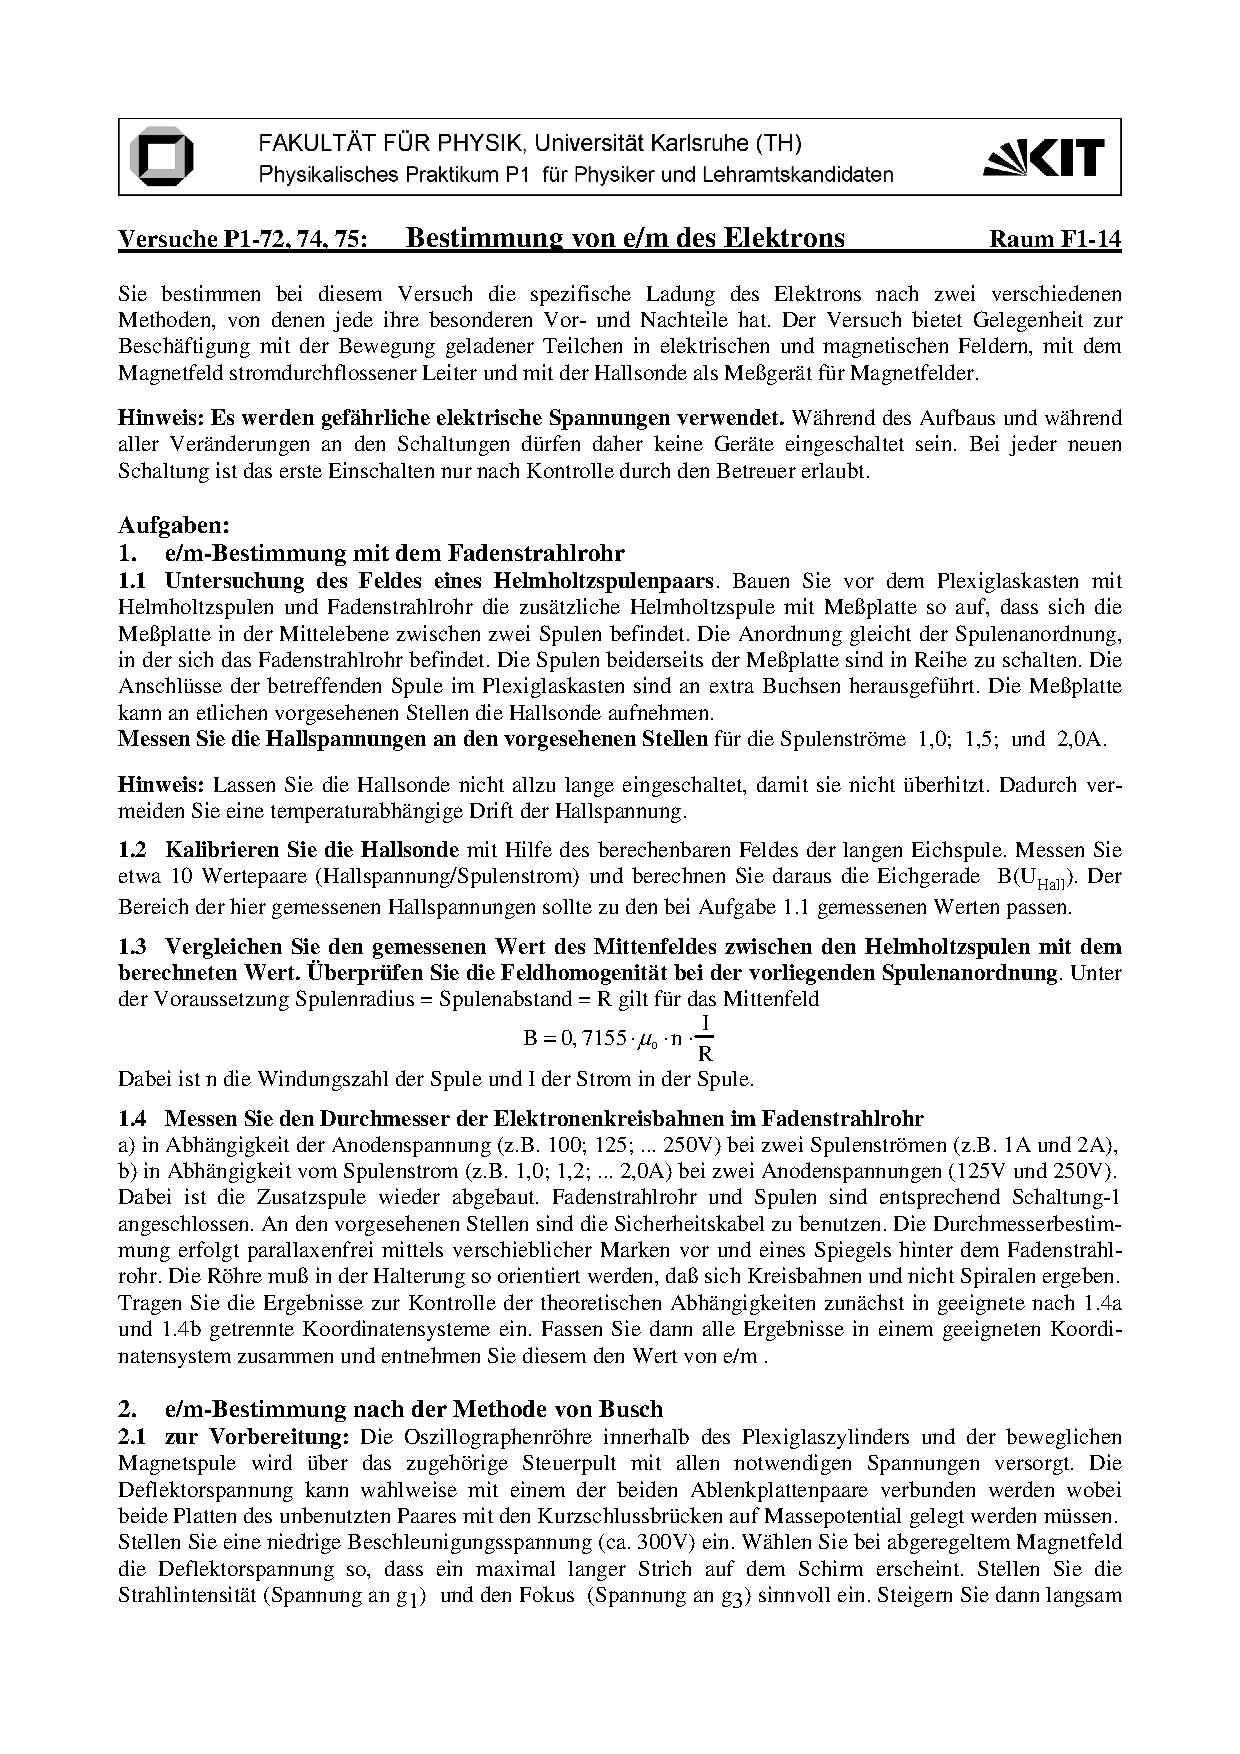
\includepdf[pages=-,scale=0.8]{./include/EdurchM-Bestimmung.pdf}
\begin{center}                                       
  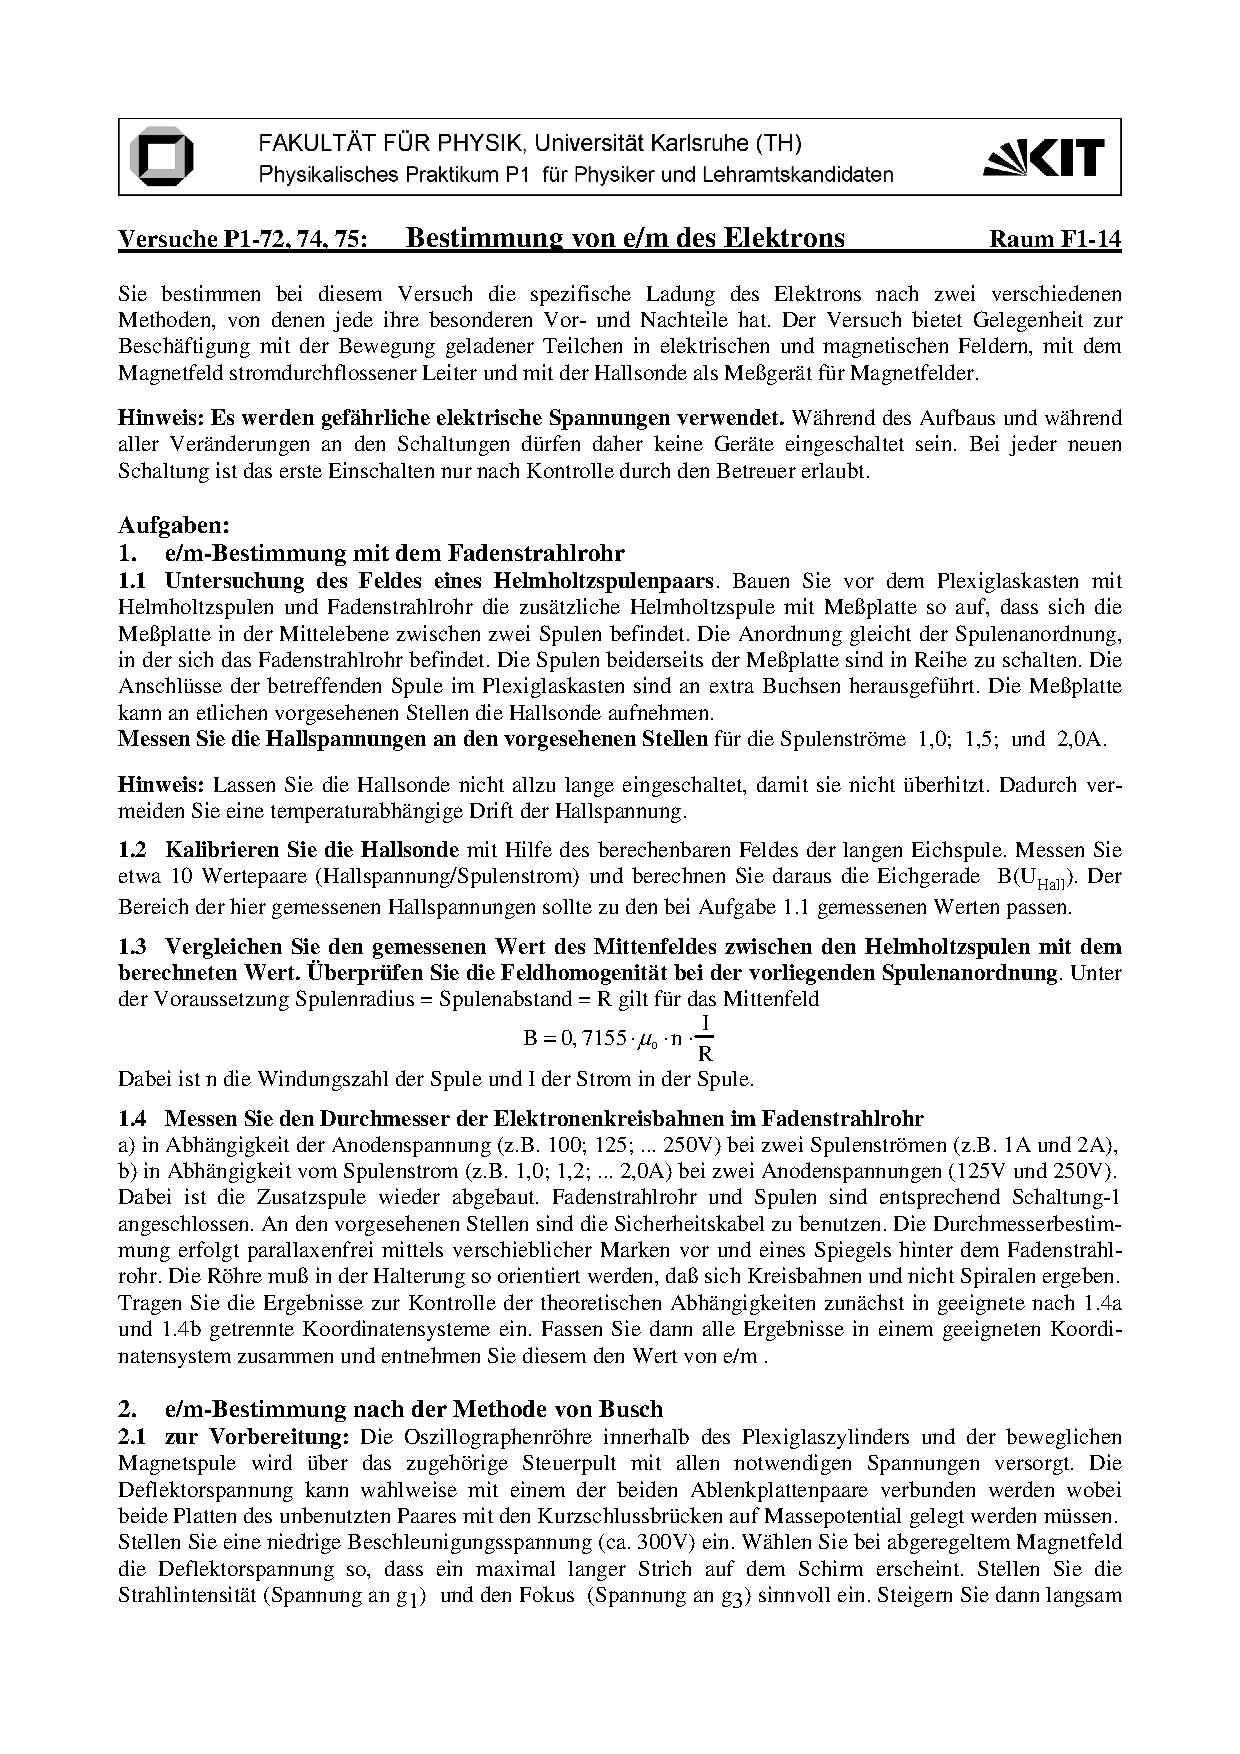
\includegraphics[
    page={1},
    width=1.1\textwidth,
    height=1.1\textheight,
]{./include/EdurchM-Bestimmung.pdf} 
      
  \includegraphics[
    page={2},
    width=1.1\textwidth,
    height=1.1\textheight,
]{./include/EdurchM-Bestimmung.pdf}                                
\end{center}                                
                                       
                                       
                                       
    \pseudochapter[3]{Messprotokoll}  % usage: \pseudochapter[number of pages 
                                        %        added]{name of the chapter}
    
 \chapter{Einleitung}
\label{Einleitung}
In dem durchgeführten Versuch wird mittels eines Fadenstrahlrohres und der Methode von Busch die spezifische Elektronenladung bestimmt. 

Bei der Bestimmung mittels Fadenstrahlrohr (siehe Kapitel \ref{HemholtzspulenpaarUntersuchung}) wird ausgenutzt, dass Elektronen im Magnetfeld aufgrund der Lorentzkraft eine Kreisbahn bilden und bei Kollision mit dem Wasserstoffgasmolekülen Photonen abgeben, welche wiederum als leuchtender Elektronenstrahl sichtbar werden [ref].

Hingegen wird bei der Methode von Busch (siehe Kapitel \ref{MethodeBusch}) eine Braun'sche Röhre verwendet, bei welcher die Elektronen von der Kathode zur Anodode beschleunigt und auf einem Leuchtschirm auftreffen. Mit geeigneter Beschleunigungsspannung und Spulenstrom kann die spezifische Elektronenladung bestimmt werden.

Mit Hilfe der beiden Methoden wird ein Wert für die spezifische Elektronenladung ermittelt, mit dem Literaturwert($1.759*10^{11}\frac{C}{kg}$) verglichen und potentielle Fehlerquelle diskutiert.
%% https://lp.uni-goettingen.de/get/text/1545 %\cleardoublepage    
    
    \chapter{e/m-Bestimmung mit dem Fadenstrahlrohr}
\label{emBestimmung}
\section{Untersuchung des Feldes eines Helmholtzspulenpaars}
\label{HemholtzspulenpaarUntersuchung}
Um die Hallspannung zu bestimmen, bauten wir die zusätzliche Helmholtzspule mit Messplatte entsprechend der Aufgabenbeschreibung auf. Anschließend führten wir einen Nullabgleich der Hallsonde durch um den vorherrschenden geomagnetischen Feldern als auch anderen Störeinflüsse während der Messung entgegen zu wirken. Hier stellten wir bereits fest, dass kleinste Berührungen an den Messgeräten, Kabeln und anderen Anschlüssen den Nullabgleich leicht veränderten, weshalb wir bei jedem Umbau während der Abarbeitung der einzelnen Versuche, vor jeder neuen Messreihe erneut einen Nullabgleich durchführten. Wir stellten ebenso fest, dass das digitale Strommessgerät keinen konstanten Wert anzeigte und dieser während des Versuchs abnahm. Dieses Phänomen können wir nicht erklären. Vermutlich ist es durch die systematischen Fehler des Messgeräts aufgetreten. Außerdem mussten wir feststellen, dass das analoge Spannungsmessgerät ähnliche Fehler hatte.   

\begin{figure}[hbtp]
\centering
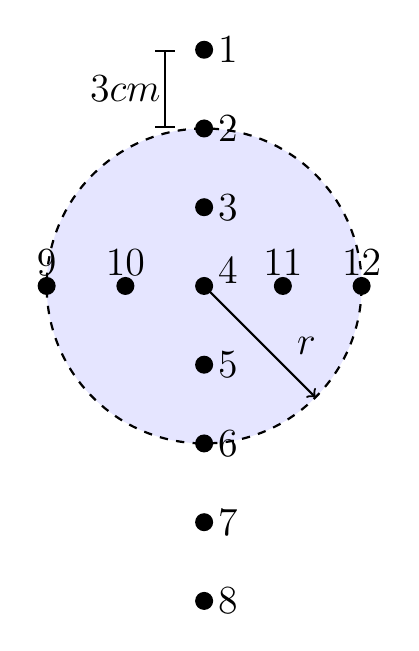
\begin{tikzpicture}[style={font=\Large}]
%\draw[thick,dashed] (0,0) circle (4cm);
\filldraw[fill=blue!10!white,thick,dashed] (0,0) circle (2cm);
\draw[|-|,thick] (-0.5,2) -- (-0.5, 3)node at (-1,2.5) {\textbf{$3cm$}};
\draw[->,thick] (0,0) -- (1.41421356, -1.41421356)node at (1.3,-1)[above] {\textbf{$r$}};
\draw[thick,fill] (0,3) circle (0.1cm) node at (0.3,3)[] {\textbf{$1$}};
\draw[thick,fill] (0,2) circle (0.1cm) node at (0.3,2)[] {\textbf{$2$}};
\draw[thick,fill] (0,1) circle (0.1cm) node at (0.3,1)[] {\textbf{$3$}};
\draw[thick,fill] (0,0) circle (0.1cm) node at (0.3,0.2)[] {\textbf{$4$}};
\draw[thick,fill] (0,-1) circle (0.1cm) node at (0.3,-1)[] {\textbf{$5$}};
\draw[thick,fill] (0,-2) circle (0.1cm) node at (0.3,-2)[] {\textbf{$6$}};
\draw[thick,fill] (0,-3) circle (0.1cm) node at (0.3,-3)[] {\textbf{$7$}};
\draw[thick,fill] (0,-4) circle (0.1cm) node at (0.3,-4)[] {\textbf{$8$}};
\draw[thick,fill] (-2,0) circle (0.1cm) node at (-2,0.3)[] {\textbf{$9$}};
\draw[thick,fill] (-1,0) circle (0.1cm) node at (-1,0.3)[] {\textbf{$10$}};
\draw[thick,fill] (1,0) circle (0.1cm) node at (1,0.3)[] {\textbf{$11$}};
\draw[thick,fill] (2,0) circle (0.1cm) node at (2,0.3)[] {\textbf{$12$}};
\end{tikzpicture}
\caption{Verwendeten Messplatte mit Umgebung des homogenen Magnetfeldes}
\label{fig:MessPlatte}
\end{figure}

Entsprechend Anweisung seitens unserer Betreuerin, als auch den Hinweisen der Aufgabenbeschreibung maßen wir den ersten und höchsten Ausschlag der Hallspannung für die jeweilige Spulenströme von $1 A$, $1.5 A$ und $2 A$ an den vorgegebenen Positionen der Messplatte (siehe Abbildung \ref{fig:MessPlatte}). Aufgrund der zuvor erwähnten  Empfindlichkeit der  Hallsonde führten wir die Messung für $1 A$ erneut durch, da diese anfangs uns falsch erschienen.


\newpage
 

\begin{table}
\begin{center}
\begin{tabular}{|c|c|c|c|}
\hline 
& I = 1 A & I = 1.5 A & I = 2 A \\ 
\hline 
Punkt & $U_h$ [mV] & $U_h$ [mV] & $U_h$ [mV] \\ 
\hline 
1 & 0.105 & 0.16 & 0.2 \\ 
\hline 
2 & 0.112 & 0.165 & 0.21 \\ 
\hline 
3 & 0.112 & 0.165 & 0.215 \\ 
\hline 
4 & 0.112 & 0.165 & 0.215 \\ 
\hline 
5 & 0.112 & 0.165 & 0.215 \\ 
\hline 
6 & 0.112 & 0.16 & 0.21 \\ 
\hline 
7 & 0.106 & 0.15 & 0.2 \\ 
\hline 
8 & 0.087 & 0.12 & 0.165 \\ 
\hline 
9 & 0.108 & 0.16 & 0.21 \\ 
\hline 
10 & 0.108 & 0.16 & 0.215 \\ 
\hline 
11 & 0.108 & 0.16 & 0.215 \\ 
\hline 
12 & 0.11 & 0.16 & 0.21 \\ 
\hline 
\end{tabular} 
\caption{Hallspannungen der Helmnholzspulenpaares}
\end{center}
\end{table}

\begin{center}                                       
  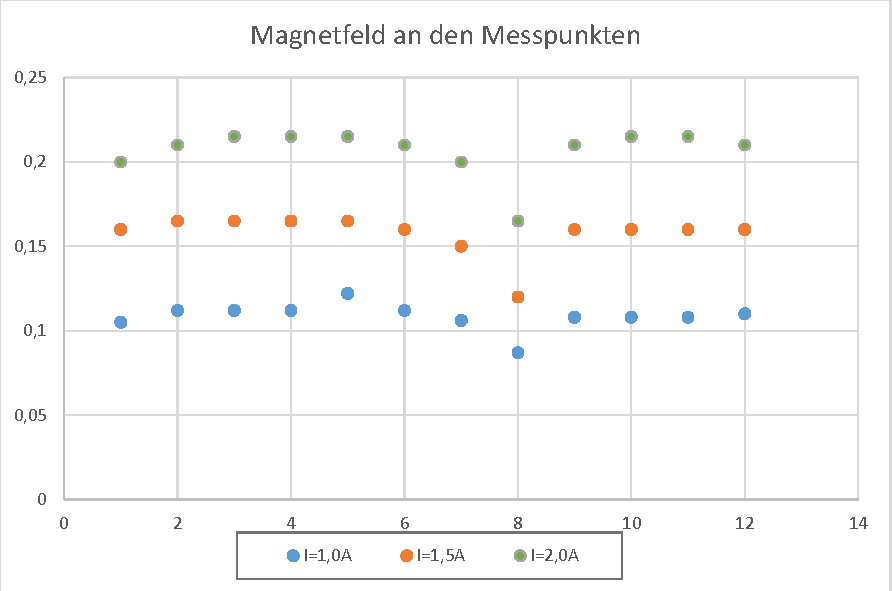
\includegraphics{./include/Bfeld.pdf} 
                          
\end{center} 

TABELLE MIT WERTEN IN ANHANG

Abbildung BFELD zeigt die magnetische Flussdichte abhängig von den Messpunkten. Zu sehen ist, dass das Feld im Radius von $6 cm$ um den Punkt 4 recht homogen ist (siehe Abbildung \ref{fig:Bfeld}). Dieser Aspekt lässt sich mit den Eigenschaften des Helmholtzspulenpaares bezüglich der Feldhomogenität vereinbaren. Außerdem ist ein deutlicher Abfall der magnetischen Flussdichte im Punkt 8 zu sehen, da dieser außerhalb des Radius liegt

\section{Kalibrieren der Hallsonde}
Um die Hallsonde möglichst genau zu Eichen wurde sie in die Mitte der Spule eingeführt und zehn Messungen der Hallspannung durchgeführt. Anhand der Formel für lange Spulen:
\begin{equation*}
B_{spule} = \mu_0 \cdot \frac{n \cdot I}{L}
\end{equation*}
kann die magnetische Flussdichte der Spule bestimmt werden. Die Maßzahlen der Eichspulen sind L = 300mm, d = 20 mm, n = 750 Windungen. Für die magnetische Feldkonstante $\mu_0$ wurde der Literaturwert $4\pi \cdot 10^{-7} \frac{N}{A^2}$ verwendet.
%https://lp.uni-goettingen.de/get/text/4087

Um die Eichgerade zu bestimmen wird das Gleichgewicht zwischen der Lorentzkraft und der elektrischen Kraft ausgenutzt:
\begin{eqnarray*}
F_{lorentz} &=& F_{elektrisch} \\
q \cdot v \cdot B_{spule} &=& q \cdot E \quad | \quad E = \frac{U_h}{d}\\
B_{spule} &=&\frac{1}{v \cdot d} \cdot U_h \Rightarrow m = \frac{1}{v \cdot d}
\end{eqnarray*}
Somit lässt sich ein linearer Zusammenhang zwischen Hallspannung und magnetischen Flussdichte herstellen. Die Steigung $m$ ist nur von der Spannung der Hallsonde abhängig und somit konstant. Sie lässt sich aus den gemessenen Hallspanungen und berechneten Flussdichten (siehe Tabelle \ref{tab:eichspule}) mit linearer Regression (siehe Abbildung \ref{tab:eichspule}) berechnen und liegt bei $m = 0.146 \frac{s}{m^2}$. Außerdem stimmen die gemessenen Hallspannungen etwa mit den Messungen aus Kapitel \ref{HemholtzspulenpaarUntersuchung} überein.

\begin{minipage}[h]{0.35\linewidth}

\begin{tabular}{|c|c|c|}
\hline 
I [A] & $U_h$ [mV] & $B_{spule}$ [mT] \\ 
\hline 
0.199 & 0.094 & 0.625
 \\ 
\hline 
0.230 & 0.106 & 0.722
 \\ 
\hline 
0.287 & 0.135 & 0.901
 \\ 
\hline 
0.320 & 0.15 & 1.005
 \\ 
\hline 
0.363 & 0.17 & 1.140
 \\ 
\hline 
0.398 & 0.185 & 1.250
 \\ 
\hline 
0.445 & 0.205 & 1.398
 \\ 
\hline 
0.499 & 0.235 & 1.567
 \\ 
\hline 
0.540 & 0.25 & 1.696
 \\ 
\hline 
0.587 & 0.27 & 1.844
 \\ 
\hline 
\end{tabular} 
\captionof{table}{Berechnete magnetische Flussdichte der Eichspule}
\label{tab:eichspule}
\end{minipage}
\hfill
\begin{minipage}[h]{0.6\linewidth}

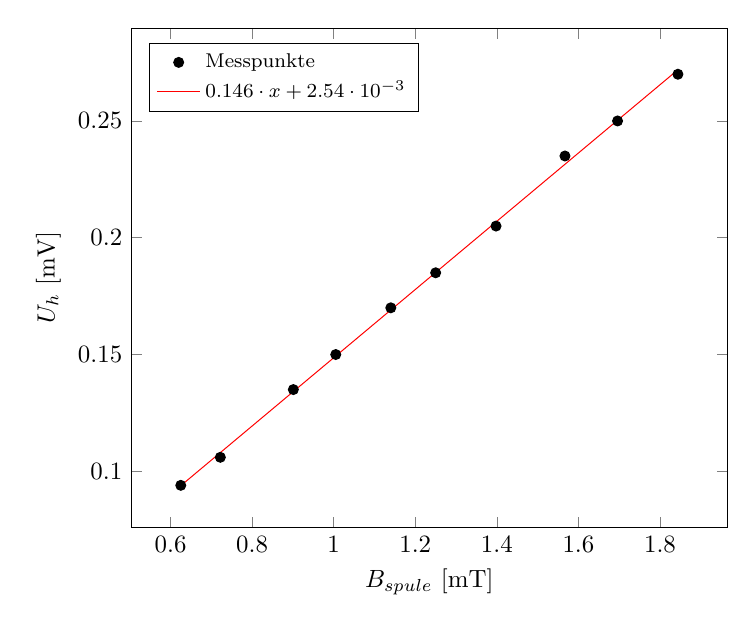
\begin{tikzpicture}[scale=0.9]
    \pgfplotsset{width=10cm,
        compat=1.10,
        legend style={font=\footnotesize}}
    \begin{axis}[
    xlabel={$B_{spule}$  [mT]},
    ylabel={$U_h$ [mV]},
    legend cell align=left,
    legend pos=north west]
    \addplot[only marks] table[row sep=\\]{
        X Y\\
 0.625   0.094\\
 0.722    0.106\\
 0.901   0.135\\
 1.005    0.15\\
 1.140   0.17\\
 1.250   0.185\\
 1.398    0.205\\
 1.567   0.235\\
 1.696    0.25\\
 1.844   0.27\\
    };
    \addlegendentry{Messpunkte}
    \addplot[no markers,red] table[row sep=\\,
    y={create col/linear regression={y=Y}}] % compute a linear regression from the
    %input table
    {
        X Y\\
 0.625   0.094\\
 0.722    0.106\\
 0.901   0.135\\
 1.005    0.15\\
 1.140   0.17\\
 1.250   0.185\\
 1.398    0.205\\
 1.567   0.235\\
 1.696    0.25\\
 1.844   0.27\\
    };
    \addlegendentry{%
        $\pgfmathprintnumber[precision=3]{\pgfplotstableregressiona} \cdot x
        \pgfmathprintnumber[print sign]{\pgfplotstableregressionb}$} %
    \end{axis}
\end{tikzpicture}
\captionof{figure}{Eichspulengerade}
\label{fig:Eichspulengerade}
\end{minipage}

	

    

\section{Vergleich zwischen gemessenen und berechneten Wert des Mittenfeldes zwischen den Helmholtzspulen}
Um die Genauigkeit unserer Messwerte und dem daraus berechneten Magnetfeld zu überprüfen haben wir für die drei Stromstärken $1 A$,$1.5 A$, und $2 A$ unseren gemessenen als auch den Soll-Wert vergleichen. Die Abweichungen vom Sollwert sind in Prozent angegeben.
 
 In XX sieht man, dass aufgrund der zuvor beschriebenen Messunsicherheiten seitens der Messgeräte (siehe Kapitel 1,111) sowie den sich fortpflanzenden Fehlern während der Nullabstimmung als auch der in 1.2 beschrieben Eichung, Abweichungen auftreten. So erhielten wir dennoch Abweichungen die noch sehr gering sind.
 
 Im Nachfolgenden wird nun mit dem Sollwert weiter gerechnet um die Fortpflanzung der zuvor beschrieben Messunsicherheiten zu vermeiden.
 
 
\section{Messung des Durchmessers der Elektronenkreisbahn im Fadenstrahlrohr}
\paragraph{In Abhängigkeit der Anodenspannung}
Entsprechend der Aufgabenbeschreibung bauten wir den Versuch auf und bestimmten für Anodenspannungen von 125V bis 250V bei jeweils 1A und 2A die zugehörigen Durchmesser der Elektronenkreisbahn. Hierfür wählten wir einen adjazenten Abstand von 25V. Parallaxenfehler bei der Bestimmung des Durchmessers wurden gemäß Anordnung möglichst klein gehalten. Jedoch stellte sich das exakte bestimmen des Durchmessers als dennoch schwierig heraus, was an dem stellenweise diffusen Elektronenstrahl zuzuschreiben ist. Um möglichst gute Ergebnisse zu erzielen überprüften wir jeweils die Bestimmung des Durchmessers des jeweils anderen. Aufgrund der zu großen Kreisbahn und demndamit überschrittenen Messbereich unserer Versuchsanordnung konnten wir bei 1A für Anodenspannungen größer als 200V keinen Durchmesser der Kreisbahn bestimmen. Hingegen konnten wir bei 2A für alle Anodenspannungen einen Durchmesser bestimmen. So ermittelten wir die in Abbildung XX gezeigten Messwerte. 




\paragraph{In Abhängigkeit des Spulenstroms}
Nun untersuchten wir entsprechend der Aufgabenbeschreibung in b die  Durchmesser der Elektronenkreisbahn für zwei feste Beschleunigungsspannungen (150V und 250V) für Spulenströme zwischen 1A bis 2A. Hierfür wählten den adjazenten Abstand von 0.2A. Auch hier trat das soeben beschriebene Problem des Diffusen Elektronenstrahls auf. Bis auf den Messwert für 1A bei 250V konnten wir für jede Konfiguration einen Durchmesser bestimmen, welche in Abbildung XX zu sehen sind.






 %\cleardoublepage
    
      \chapter{e/m-Bestimmung nach Methode von Busch}
\section{Vorbereitung des Versuchs}
Entsprechend Aufgabenbeschreibung stellten wir die Ablenkspannung und  Deflektorspannung so ein, dass wir einen maximal langen Strich erhielten.So könnten wir beobachten, dass bei Änderung der Ablenkspannung XX passiert und bei der Deflektorspannung YY. Beim Einstellen des maximal langen Strichs stellten wir fest, dass der Strich mittig unterbrochen schien bzw. weniger intensiv war. Ebenso war es schwierig mit zuvor eingestellten Messwerten einen exakten Punkt zu erzielen. Nach einigen Justierungen konnten wir einen möglichst kleinen Punkt auf dem Schirm der Kathodenstrahlen erzielen.
\section{Messung des nötigen Spulenstroms für die Beschleunigungsspannung}
Gemäß Aufgabe stellten wir die Beschleunigungsspannung auf Werte zwischen 500V und 700V. Hierfür wählten wir eine Schrittweite von 50V und führten den nötigen Spulenstrom zu, welcher nötig war um für die unterschiedlichen Beschleunigungsspannungen einen Punkt auf den Schirm zu erzielen. Die nötigen Spulenströme für die jeweiligen Beschleunigungspannungen sind in Abbildung enthalten.

 %\cleardoublepage

    % appendix for more or less interesting calculations
    \Appendix
    \chapter*{\appendixname} \addcontentsline{toc}{chapter}{\appendixname}
    % to make the appendix appear in ToC without number. \appendixname = 
    % Appendix or Anhang (depending on chosen language)
    \section{Erster Abschnitt des Anhangs}
Dies ist der erste ganz tolle Abschnitt des Anhangs. %\cleardoublepage



    % Bibliography
    \TheBibliography

    % BIBTEX
    % use if you want citations to appear even if they are not referenced to: 
    % \nocite{*} or maybe \nocite{Kon64,And59} for specific entries
    %\nocite{*}
    \bibliographystyle{babalpha}
    \bibliography{lit.bib}

    % THEBIBLIOGRAPHY
    %\begin{thebibliography}{000}
    %    \bibitem{ident}Entry into Bibliography.
    %\end{thebibliography}
\end{document}
